\chapter{Résultat}

L'application que nous avons publié est l'aboutissement du projet. Elle contient de nombreuses fonctionnalités, qui forment une base permettant l'ajout de nouveau contenu de façon simple. Dans la plupart des rapports, une partie est dédiée à un mode d'emploi. Il était important pour nous qu'il n'y ai pas besoin de lire un guide avant de jouer, cette partie n'est donc pas nécessaire. Nous avons préféré présenter le contenu résultat du jeu.

\paragraph{L'écran d'accueil} Le principe étant d'avoir un écran principal permettant d'accéder aux fonctionnalités principale de l'application. Il possède ainsi le titre de l'application, un bouton qui permet d'avoir accès à la grille des niveaux, un bouton permettant d'enlever les publicités en échange de $1,20$ euros, et enfin, un bouton qui donne les crédits à l'auteur des musiques ainsi que les noms des développeurs.

\begin{figure}[H]\centering
  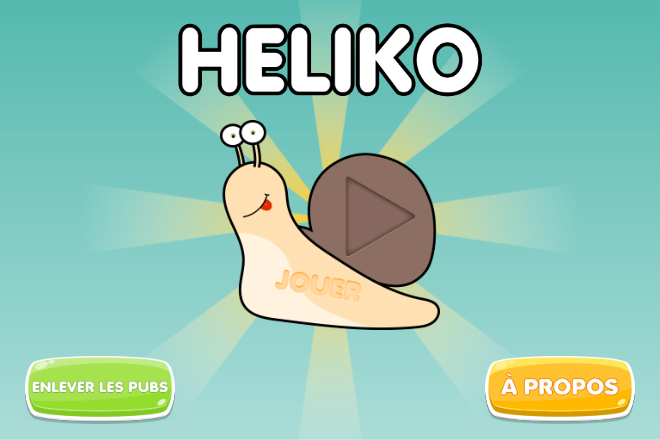
\includegraphics[scale=0.6]{./img/resultat_accueil.png}
  \caption{L'écran d'accueil de l'application}
  \label{analytics}
\end{figure}

\paragraph{Choix des niveaux} Cet écran permet à l'utilisateur de sélectionner le niveau de son choix. Au démarrage, seul un niveau est actif, les autres sont grisés et inaccessibles. Pour les débloquer, le joueur doit réussir le niveau précédent.

\begin{figure}[H]\centering
  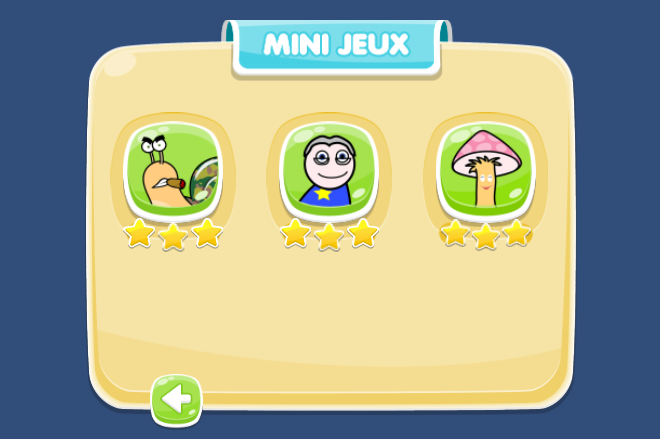
\includegraphics[scale=0.6]{./img/resultat_niveaux.png}
  \caption{L'écran de choix du niveau}
  \label{analytics}
\end{figure}

Ce menu permet aussi d'afficher le nombre d'étoiles obtenues sur chaque niveau. L'utilisateur peut ainsi facilement retrouver les niveaux qu'il n'a pas encore réussi à 100\%.

\paragraph{Le menu pause}

A n'importe quel moment de n'importe quel mini-jeu, le joueur peut décider de mettre en pause sa partie. Ce menu permet de reprendre la partie au moment où le bouton pause a été pressé, de recommencer le jeu en cours depuis le début, ou bien de quitter le niveau pour revenir à l'écran de sélection.

\paragraph{L'écran de fin de partie}

A la fin d'un mini-jeu, l'application affiche le résultat de la partie, en attribuant au joueur une note en fonction de son degré de réussite sur le niveau, ainsi qu'une rapide appréciation. Il propose ensuite un bouton pour recommencer le niveau et un autre pour retourner à l'accueil.

\section*{Les mini-jeux}

\paragraph{La marche de l'escargot}

Ce mini-jeu est proposé en premier car sa difficulté est faible. Il consiste à suivre le rythme de la musique et de taper en même temps que les coups de trompette qui battent la mesure. Le motif à jouer est répétitif et n'est donc pas compliqué à mémoriser.

\begin{figure}[H]\centering
  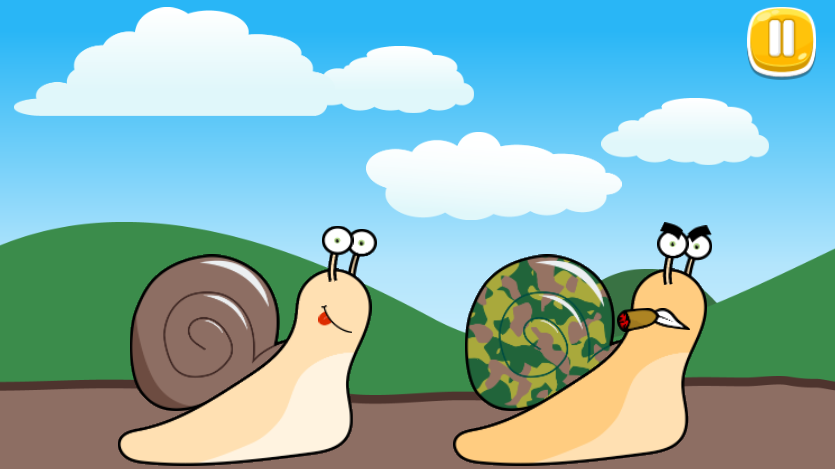
\includegraphics[scale=0.4]{./img/resultat_escargot.png}
  \caption{Le niveau de la Marche des escargots}
  \label{analytics}
\end{figure}

Lors de l'échec, un son différent est joué, et le sergent-escargot n'est pas content !


\paragraph{Le magicien}

La difficulté de ce niveau est plus élevée et repose sur l'action de maintenir le doigt sur l'écran pendant un temps précis. Lorsque l'objet apparait au-dessus du chapeau du magicien, le joueur doit appuyer sur l'écran pour l'abaisser dans le chapeau. En fonction de l'objet, il doit rester appuyé un certain temps, puis relâcher lorsque ce temps est terminé. S'il réussit, l'objet sera transformé en un autre contenant le même jeu de couleurs, sinon un escargot triste apparaitra et un son triste sera joué. La durée pendant laquelle il faut maintenir l'objet dans le chapeau est indiqué dans le tutoriel en début de partie.

\begin{figure}[H]\centering
  
\includegraphics[scale=0.5]{./img/resultat_magicien.png}
  \caption{Le niveau du magicien}
  \label{analytics}
\end{figure}

Ce niveau comporte des effets de particules pour renforcer l'aspect magique de l'ambiance.

\paragraph{Les champignons}

Malgré le fait que ce niveau ai été développé en premier, il se retrouve en dernier dans la liste des mini-jeux proposés. Cela est dû à sa difficulté qui est élevée. En effet, pour le réussir, il faut avoir déjà pris l'habitude de battre le rythme sur son smartphone au travers des autres jeux. De plus l'attention du joueur doit être totale pendant toute la durée du jeu.

\begin{figure}[H]\centering
  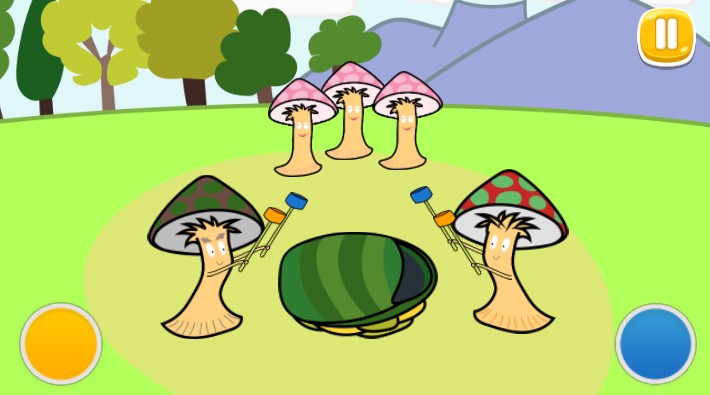
\includegraphics[scale=0.5]{./img/resultat_champis.png}
  \caption{Le niveau des champignons}
  \label{analytics}
\end{figure}

Le principe consiste à répéter à l'identique l'action du papi-champignon, après que celui-ci nous donne le signal. Le joueur est représenté par un champignon plus jeune, et donne ainsi l'impression de recevoir des instruction d'un grand sage champignon. Des champignons fans sont présents en arrière plan et battent la mesure de la musique. La difficulté est croissante au fur et à mesure de l'avancée du niveau, ainsi au début du jeu seuls les temps pleins sont joués, puis on rajoute des demi-temps et même des quarts de temps. Le tutoriel permet de s'initier au jeu en douceur.
